\documentclass[12pt, fullpage,letterpaper]{article}

\usepackage[margin=1in]{geometry}
\usepackage{url}
\usepackage{amsmath}
\usepackage{amssymb}
\usepackage{xspace}
\usepackage{graphicx}
\graphicspath{ {Images/} }


\newcommand{\semester}{Spring 2018}
\newcommand{\assignmentId}{4}
\newcommand{\releaseDate}{11 April, 2018}
\newcommand{\dueDate}{23 April, 2018}

\newcommand{\bx}{{\bf x}}
\newcommand{\bw}{{\bf w}}

\title{CS 5350/6350: Machine Learining \semester}
\author{Homework \assignmentId}
\date{Handed out: \releaseDate\\
  Due date: \dueDate}

\begin{document}
\maketitle

% Math commands by Thomas Minka
\newcommand{\var}{{\rm var}}
\newcommand{\Tr}{^{\rm T}}
\newcommand{\vtrans}[2]{{#1}^{(#2)}}
\newcommand{\kron}{\otimes}
\newcommand{\schur}[2]{({#1} | {#2})}
\newcommand{\schurdet}[2]{\left| ({#1} | {#2}) \right|}
\newcommand{\had}{\circ}
\newcommand{\diag}{{\rm diag}}
\newcommand{\invdiag}{\diag^{-1}}
\newcommand{\rank}{{\rm rank}}
% careful: ``null'' is already a latex command
\newcommand{\nullsp}{{\rm null}}
\newcommand{\tr}{{\rm tr}}
\renewcommand{\vec}{{\rm vec}}
\newcommand{\vech}{{\rm vech}}
\renewcommand{\det}[1]{\left| #1 \right|}
\newcommand{\pdet}[1]{\left| #1 \right|_{+}}
\newcommand{\pinv}[1]{#1^{+}}
\newcommand{\erf}{{\rm erf}}
\newcommand{\hypergeom}[2]{{}_{#1}F_{#2}}

% boldface characters
\renewcommand{\a}{{\bf a}}
\renewcommand{\b}{{\bf b}}
\renewcommand{\c}{{\bf c}}
\renewcommand{\d}{{\rm d}}  % for derivatives
\newcommand{\e}{{\bf e}}
\newcommand{\f}{{\bf f}}
\newcommand{\g}{{\bf g}}
\newcommand{\h}{{\bf h}}
%\newcommand{\k}{{\bf k}}
% in Latex2e this must be renewcommand
\renewcommand{\k}{{\bf k}}
\newcommand{\m}{{\bf m}}
\newcommand{\mb}{{\bf m}}
\newcommand{\n}{{\bf n}}
\renewcommand{\o}{{\bf o}}
\newcommand{\p}{{\bf p}}
\newcommand{\q}{{\bf q}}
\renewcommand{\r}{{\bf r}}
\newcommand{\s}{{\bf s}}
\renewcommand{\t}{{\bf t}}
\renewcommand{\u}{{\bf u}}
\renewcommand{\v}{{\bf v}}
\newcommand{\w}{{\bf w}}
\newcommand{\x}{{\bf x}}
\newcommand{\y}{{\bf y}}
\newcommand{\z}{{\bf z}}
%s\newcommand{\l}{\boldsymbol{l}}
\newcommand{\A}{{\bf A}}
\newcommand{\B}{{\bf B}}
\newcommand{\C}{{\bf C}}
\newcommand{\D}{{\bf D}}
\newcommand{\E}{{\bf E}}
\newcommand{\F}{{\bf F}}
\newcommand{\G}{{\bf G}}
\renewcommand{\H}{{\bf H}}
\newcommand{\I}{{\bf I}}
\newcommand{\J}{{\bf J}}
\newcommand{\K}{{\bf K}}
\renewcommand{\L}{{\bf L}}
\newcommand{\M}{{\bf M}}
\newcommand{\N}{\mathcal{N}}  % for normal density
%\newcommand{\N}{{\bf N}}
\renewcommand{\O}{{\bf O}}
\renewcommand{\P}{{\bf P}}
\newcommand{\Q}{{\bf Q}}
\newcommand{\R}{{\bf R}}
\renewcommand{\S}{{\bf S}}
\newcommand{\T}{{\bf T}}
\newcommand{\U}{{\bf U}}
\newcommand{\V}{{\bf V}}
\newcommand{\W}{{\bf W}}
\newcommand{\X}{{\bf X}}
\newcommand{\Y}{{\bf Y}}
\newcommand{\Z}{{\bf Z}}

% this is for latex 2.09
% unfortunately, the result is slanted - use Latex2e instead
%\newcommand{\bfLambda}{\mbox{\boldmath$\Lambda$}}
% this is for Latex2e
\newcommand{\bfLambda}{\boldsymbol{\Lambda}}

% Yuan Qi's boldsymbol
\newcommand{\bsigma}{\boldsymbol{\sigma}}
\newcommand{\balpha}{\boldsymbol{\alpha}}
\newcommand{\bpsi}{\boldsymbol{\psi}}
\newcommand{\bphi}{\boldsymbol{\phi}}
\newcommand{\boldeta}{\boldsymbol{\eta}}
\newcommand{\Beta}{\boldsymbol{\eta}}
\newcommand{\btau}{\boldsymbol{\tau}}
\newcommand{\bvarphi}{\boldsymbol{\varphi}}
\newcommand{\bzeta}{\boldsymbol{\zeta}}

\newcommand{\blambda}{\boldsymbol{\lambda}}
\newcommand{\bLambda}{\mathbf{\Lambda}}
\newcommand{\bOmega}{\mathbf{\Omega}}
\newcommand{\bomega}{\mathbf{\omega}}
\newcommand{\bPi}{\mathbf{\Pi}}

\newcommand{\btheta}{\boldsymbol{\theta}}
\newcommand{\bpi}{\boldsymbol{\pi}}
\newcommand{\bxi}{\boldsymbol{\xi}}
\newcommand{\bSigma}{\boldsymbol{\Sigma}}

\newcommand{\bgamma}{\boldsymbol{\gamma}}
\newcommand{\bGamma}{\mathbf{\Gamma}}

\newcommand{\bmu}{\boldsymbol{\mu}}
\newcommand{\1}{{\bf 1}}
\newcommand{\0}{{\bf 0}}

% \newcommand{\comment}[1]{}

\newcommand{\bs}{\backslash}
\newcommand{\ben}{\begin{enumerate}}
\newcommand{\een}{\end{enumerate}}

 \newcommand{\notS}{{\backslash S}}
 \newcommand{\nots}{{\backslash s}}
 \newcommand{\noti}{{\backslash i}}
 \newcommand{\notj}{{\backslash j}}
 \newcommand{\nott}{\backslash t}
 \newcommand{\notone}{{\backslash 1}}
 \newcommand{\nottp}{\backslash t+1}
% \newcommand{\notz}{\backslash z}

\newcommand{\notk}{{^{\backslash k}}}
%\newcommand{\noti}{{^{\backslash i}}}
\newcommand{\notij}{{^{\backslash i,j}}}
\newcommand{\notg}{{^{\backslash g}}}
\newcommand{\wnoti}{{_{\w}^{\backslash i}}}
\newcommand{\wnotg}{{_{\w}^{\backslash g}}}
\newcommand{\vnotij}{{_{\v}^{\backslash i,j}}}
\newcommand{\vnotg}{{_{\v}^{\backslash g}}}
\newcommand{\half}{\frac{1}{2}}
\newcommand{\msgb}{m_{t \leftarrow t+1}}
\newcommand{\msgf}{m_{t \rightarrow t+1}}
\newcommand{\msgfp}{m_{t-1 \rightarrow t}}

\newcommand{\proj}[1]{{\rm proj}\negmedspace\left[#1\right]}
\newcommand{\argmin}{\operatornamewithlimits{argmin}}
\newcommand{\argmax}{\operatornamewithlimits{argmax}}

\newcommand{\dif}{\mathrm{d}}
\newcommand{\abs}[1]{\lvert#1\rvert}
\newcommand{\norm}[1]{\lVert#1\rVert}

%miscellaneous symbols
\newcommand{\ie}{{{i.e.,}}\xspace}
\newcommand{\eg}{{{\em e.g.,}}\xspace}
\newcommand{\EE}{\mathbb{E}}
\newcommand{\VV}{\mathbb{V}}
\newcommand{\sbr}[1]{\left[#1\right]}
\newcommand{\rbr}[1]{\left(#1\right)}
\newcommand{\cmt}[1]{}


\section*{General Instructions}

{\footnotesize
  \begin{itemize}
  \item You are welcome to talk to other members of the class about
    the homework. I am more concerned that you understand the
    underlying concepts. However, you should write down your own
    solution. Please keep the class collaboration policy in mind.

  \item Feel free discuss the homework with the instructor or the TAs.

  \item Your written solutions should be brief and clear. You need to
    show your work, not just the final answer, but you do \emph{not}
    need to write it in gory detail. Your assignment should be {\bf no
      more than 10 pages}. Every extra page will cost a point.

  \item Handwritten solutions will not be accepted.

  \item The homework is due by \textbf{midnight of the due date}. Please submit
    the homework on Canvas.

  \item Some questions are marked {\bf For 6350 students}. Students
    who are registered for CS 6350 should do these questions. Of
    course, if you are registered for CS 5350, you are welcome to do
    the question too, but you will not get any credit for it.

  \end{itemize}
}

%%% Local Variables:
%%% mode: latex
%%% TeX-master: "hw"
%%% End:



\section{VC dimension}
\begin{enumerate}
\item~[25] Suppose we have a finite hypothesis space $H$%$\Hcal$.
\begin{enumerate}
%\item~[10] Suppose $|\Hcal| = 2^{10}$. What is the VC dimension of %$\Hcal$?
\item~[10] Suppose $|H| = 2^{10}$. What is the VC dimension of $H$?

    $\mathrm{VC}(H) <= \log_2(2^{10}) = 10$\\

%\item~[15] Generally, for  any finite $\Hcal$, what is $\mathrm{VC}(\Hcal)$ ?
\item~[15] Generally, for  any finite $H$, what is $\mathrm{VC}(H)$ ?

    $\mathrm{VC}(H) <= \log_2(|H|)$

\end{enumerate}
\item~[25] Prove that linear classifiers in a plane cannot shatter any $4$ distinct points.

    To show this we have to show that for any positioning of the points an adversarial can label the points in
    such a way that they cannot be shattered.

    In order to show we must show all the possible cases.

    \pagebreak
    \begin{enumerate}

    \item For case 1 where 3 points are in a line, and the $4th$ point can be anywhere. In this case when three points are in
    a line no matter where the other point is there is always a labeling that will not shatter the positioning.

    \begin{figure}[h]
        \centering
        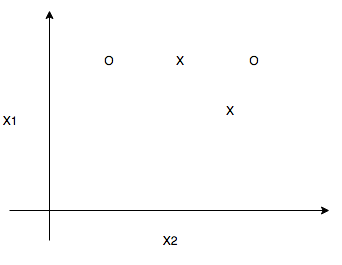
\includegraphics[scale=.5]{all_in_line.png}
    \end{figure}


    \item Then there is the second case where 3 points are not in a line, and there is two other cases that fall into
    this category.
        \begin{enumerate}
            \item Where the $4th$ point is anywhere inside a triangle of the other 3 points.
            \begin{figure}[h]
                \centering
                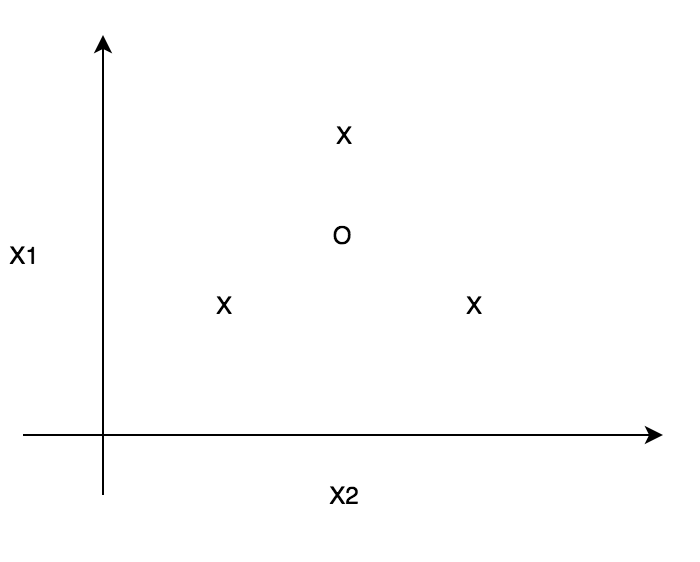
\includegraphics[scale=.5]{inside_triangle.png}
            \end{figure}
            \item Where the $4th$ point is anywhere outside of the triangle
            \begin{figure}[h]
                \centering
                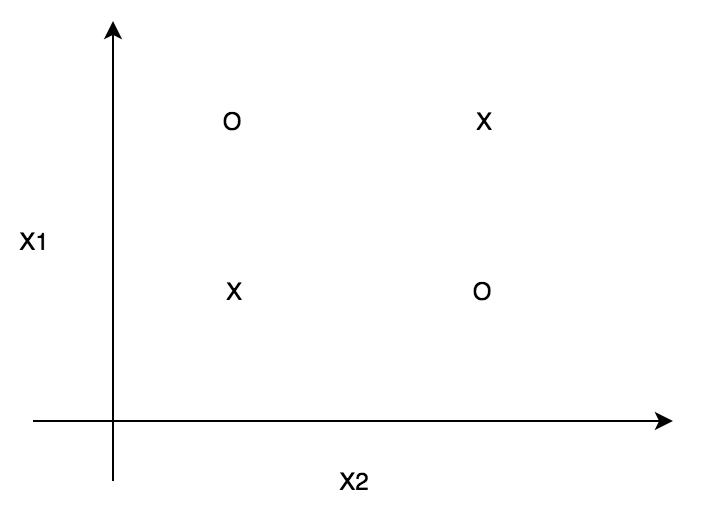
\includegraphics[scale=.5]{not_in_triangle.png}
            \end{figure}
        \end{enumerate}
    \end{enumerate}

    Since all of these are all the possible configurations we can have of the points then we can say conclude that
    lenear classifires in a plane cannot shatter any 4 distinct points.



%\item~[20] Consider our infinite hypothesis space $\Hcal$ are all rectangles in a plain. Each rectangle corresponds to a classifier --- all the points inside the rectangle are classified as positive, and otherwise classified as negative. What is $\mathrm{VC}(\Hcal)$?
\item~[20] Consider our infinite hypothesis space $H$ are all rectangles in a plain. Each rectangle corresponds to a classifier --- all the points inside the rectangle are classified as positive, and otherwise classified as negative. What is $\mathrm{VC}(H)$?\\
Infinity
\end{enumerate}

\section{Support Vector Machines}
\begin{enumerate}
\item~[20 points] Prove that the objective function of soft SVM is convex,
\[
\frac{1}{2}\w^\top\w + C\sum_{i} \max\big(0, 1 - y_i(\w^\top\x_i+b)\big).
\]

\item~[10 points] Illustrate how the Occam's Razor's principle is reflected in SVM objective function and optimization. 


%calculate the subgradient
\item~[30 points] Suppose we have the following training dataset. We want to learn a SVM classifier. We initialize all the model parameters with $0$. We set the learning rates for the first three steps to $\{0.01, 0.005, 0.0025\}$.  Please list the sub-gradients of the SVM objective w.r.t the model parameters for the first three steps, when using the stochastic sub-gradient descent algorithm. 
\begin{table}[h]
        \centering
        \begin{tabular}{ccc|c}
        $x_1$ & $x_2$ & $x_3$ &  $y$\\ 
        \hline\hline
         $0.5$ & $-1$ & $0.3$ & $1$ \\ \hline
         $-1$ & $-2$ & $-2$ & $-1$\\ \hline
         $1.5$ & $0.2$ & $-2.5$ & $1$\\ \hline
        \end{tabular}
\end{table}

\end{enumerate}

\section{Programming Assignments}
\begin{enumerate}
\item We will implement  SVM with stochastic sub-gradient descent. We will reuse the dataset for Perceptron implementation. The features and labels are listed in the file ``classification/data-desc.txt''. The training data are stored in the file ``classification/train.csv'', consisting of $872$ examples. The test data are stored in ``classification/test.csv'', and comprise of $500$ examples. In both the training and testing datasets, feature values and labels are separated by commas. Set the maximum epochs $T$ to 50. Don't forget to shuffle the training examples at the start of each epoch. Use the curve of the objective function (along with the number of updates) to diagnosis the convergence. Try the hyperparameter $C$ from $\{\frac{10}{873}, \frac{100}{873}, \frac{300}{873}, \frac{500}{873,} \frac{700}{873}\}$. Don't forget to convert the labels to be in $\{1, -1\}$.  
\begin{enumerate}
\item~[50 points] Use the schedule of learning rate: $\gamma_t = \frac{\gamma_0}{1+\frac{\gamma_0}{d}t}$. Please tune $\gamma_0$ and $d$ to ensure convergence. For each setting of $C$, report your test error. 
\item~[50 points] Use the schedule $\gamma_t = \frac{\gamma_0}{1+t}$. Report the test error for each setting of C. 
\item~[20 points] For each $C$, report the differences between the model parameters learned from the two learning rate schedules, as well as the differences between the test errors. What can you conclude? 
\end{enumerate}
\end{enumerate}

\end{document}
%%% Local Variables:
%%% mode: latex
%%% TeX-master: t
%%% End:
